\chapter{HASIL DAN PEMBAHASAN}
\label{hasil-dan-pembahasan}
Bangunan yang dijadikan objek penelitian adalah \textit{climate chamber} DTNTF FT-UGM. Dalam bab ini, akan dibahas mengenai hasil perancangan kontroler sesuai dengan langkah-langkah yang dijelaskan pada Bab IV.

\section{Model Plant JST}

Model \textit{plant} pada penelitian ini menggunakan model JST yang telah dibangun oleh Tri Hartanto\cite{skripsiTanto}. Arsitektur model dirancang dengan memperhatikan sistem \textit{plant} pada Gambar \ref{fig:5:DiagramBlokPlant}. Arsitektur memiliki nilai-nilai \textit{hyperparameter} yang dirangkum pada Tabel \ref{tbl:5:NNPlantTanto}.

\begin{figure}[!h]
	\centering
	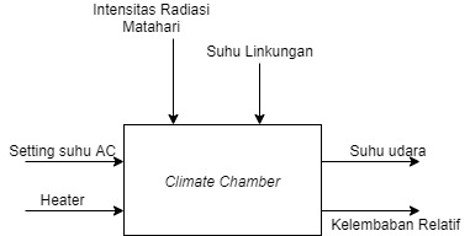
\includegraphics[width=0.5\textwidth]{figures/BlokDiagramPlant}
	\caption{Diagram Blok Plant}
	\label{fig:5:DiagramBlokPlant}
\end{figure}

\begin{figure}[!h]
	\centering
	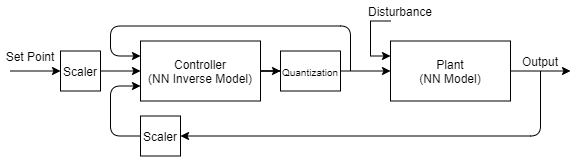
\includegraphics[width=0.85\textwidth]{figures/ControlDesignDiagramII}
	\caption{Diagram blok sistem kontrol berbasis JST}
	\label{fig:5:ConstrolSystemBlockDiagram}
\end{figure}

\begin{table}[!h]
	\caption{Tabel Rancangan Model Plant JST\cite{skripsiTanto}}
	\label{tbl:5:NNPlantTanto}
	\centering
	% use packages: array
	\begin{tabular}{|p{5cm}|p{5.2cm}|}
		\hline
		\textbf{Nama Hyperparameter} & \textbf{Nilai Hyperparameter} \\ \hline
		Arsitektur & Feedforward Neural Network \\ \hline
		Pembagian Data & 50\% 25\% 25\% \\ \hline 
		Jumlah Layar Tersembunyi & 1 \\ \hline
		Jumlah Neuron pada Layar & [55] \\ \hline
		Fungsi Aktivasi Layar & Hyperbolic Tangent \\ \hline
		Algoritma Pembelajaran & Levenberg-Marquardt \\ \hline
		Mean Absolute Error (MAE) & Tdb: 0,59$^\circ$C ; RH: 5,44\% \\ \hline
		Mean Squared Error (MSE) & Tdb: 0,75$^\circ$C ; RH: 52,33\% \\ \hline
		Koefisien Korelasi (R) & Tdb: 96,23\% ; RH: 68,90\% \\ \hline
	\end{tabular}
\end{table}

\section{Rancangan Kontrol berbasis JST}

Model JST kontroler dibangun dengan menggunakan model jaringan saraf tiruan arsitektur \textit{feedforward neural network} dengan 1 lapisan tersembunyi. Pada Sub Bab ini akan dijabarkan hasil dari proses perancangan model JST untuk kontroler.

\subsection{Variasi Pembagian Data Perancangan JST Kontroler}

Variasi pembagiaan data dilakukan dengan membandingkan beberapa variasi pembagiaan data ke dalam 5 variasi. Kemudian kinerja dari setiap pembagian data dibandingkan dengan konfigurasi hyperparameter pada Tabel \ref{tbl:5:NeuronVariation}.\\

\begin{table}[!h]
	\caption{Tabel Daftar Variasi Pembagian Data}
	\label{tbl:5:NeuronVariation}
	\centering
	% use packages: array
	\begin{tabular}{|p{3.2cm}|p{3cm}|}
		\hline
		\textbf{Pembagian Data} & \textbf{Persentase Data} \\ \hline
		Pembagian Data 1 & (50\% 25\% 25\%) \\ \hline
		Pembagian Data 2 & (60\% 20\% 20\%) \\ \hline
		Pembagian Data 3 & (70\% 15\% 15\%) \\ \hline
		Pembagian Data 4 & (80\% 10\% 10\%) \\ \hline
		Pembagian Data 5 & (80\% 15\% 05\%) \\ \hline
	\end{tabular}
\end{table}
\vspace{2em}

Model JST untuk membandingkan variasi pembagian data menggunakan arsitektur \textit{feedforward network} dengan 1 lapisan tersembunyi berisi 10 neuron. Pada tabel yang disajikan, pembagian data ditulis dengan format ’Pembagian Data n’ dan ’(x\% y\% z\%)’ dimana n = nomor variasi, x = pembagian data pelatihan, y = pembagian data validasi, dan z = pembagian data pengujian. Berdasarkan hasil variasi yang ditunjukkan pada Gambar \ref{fig:5:DataSplittingVariation}, didapatkan pembagian data terbaik yaitu pembagian data bernama "Pembagian Data 4". Data dibagi menjadi 3 bagian, yakni 80\% data pelatihan, 10\% data validasi, dan 10\% data pengujian.

\begin{figure}[!h]
	\centering
	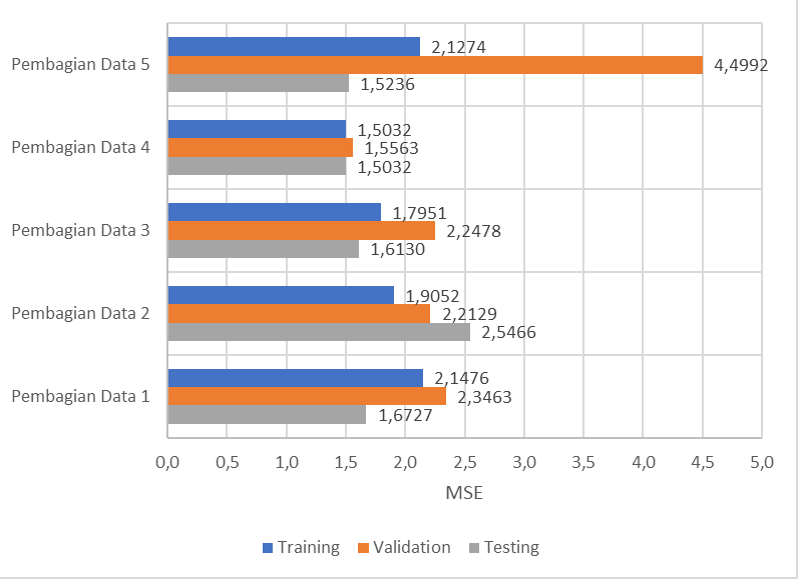
\includegraphics[width=0.85\textwidth]{figures/VariasiPembagianDataJSTKontroler}
	\caption{Grafik Variasi Pembagian Data}
	\label{fig:5:DataSplittingVariation}
\end{figure}

\subsection{Variasi Arsitektur Perancangan JST Kontroler}

Pada perancangan model JST kontroler digunakan 2 variasi fungsi aktivasi, yaitu fungsi tansig (fungsi \textit{hyperbolic tanget}) dan fungsi logsig (fungsi sigmoid). Kemudian masing-masing dilatih dengan jumlah neuron yang bervariasi dari 5 neuron hingga 60 neuron dengan lompatan sebesar 5 neuron. Dari proses variasi ini, didapatkan hasil bahwa model yang menggunakan fungsi aktivasi tansig dengan 35 neuron menghasilkan kinerja dengan nilai MSE terkecil. Hasil dari variasi ini ditunjukkan pada Gambar \ref{fig:5:ActivationVariation}.

\begin{figure}[!h]
	\centering
	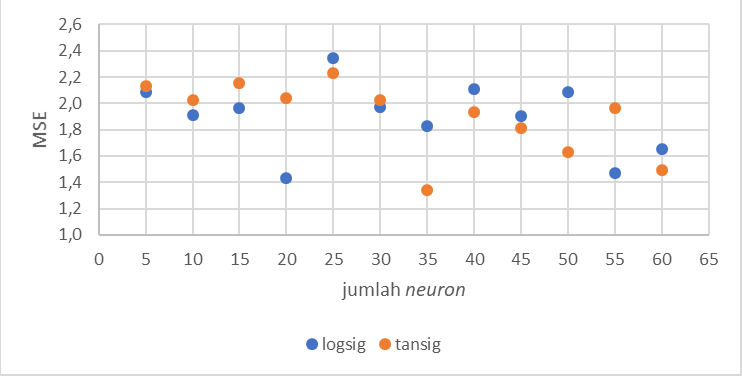
\includegraphics[width=0.75\textwidth]{figures/ActivationVariation}
	\caption{Grafik Persebaran MSE Variasi Arsitektur JST Kontroler}
	\label{fig:5:ActivationVariation}
\end{figure}

Kemudian arsitektur JST divariasikan kembali menggunakan fungsi aktivasi tansig dari 30 neuron hingga 40 neuron dengan lompatan sebesar 1 neuron untuk mengetahui kinerja model pada jumlah neuron yang berdekatan. Setelah dilakukan variasi, didapatkan hasil bahwa model JST dengan 35 neuron masih merupakan model arsitektur terbaik dengan nilai MSE terkecil. Hasil variasi ini dapat dilihat pada Gambar \ref{fig:5:NeuronVariation}.

\begin{figure}[!h]
	\centering
	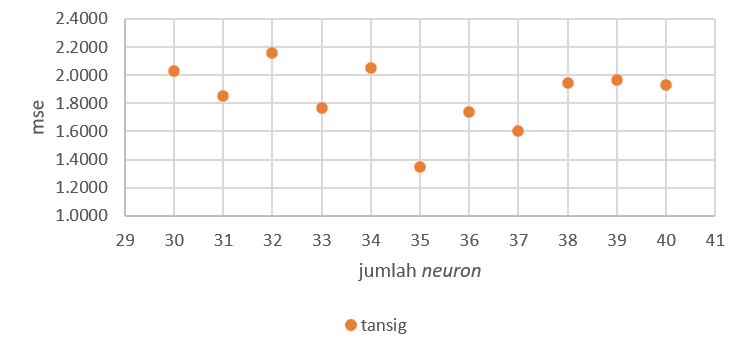
\includegraphics[width=0.75\textwidth]{figures/NeuronVariation}
	\caption{Grafik Persebaran MSE Variasi Arsitektur JST Kontroler}
	\label{fig:5:NeuronVariation}
\end{figure}

\subsection{Rancangan Model JST Kontroler}

Setelah dilakukan perancangan model JST melalui variasi arsitektur model, didapatkan rancangan model JST kontroler terbaik. Model JST dibangun dengan arsitektur \textit{feedforward neural network} 1 lapisan tersembunyi dengan 35 neuron. Model JST menggunakan fungsi aktivasi tansig (\textit{hyperbolic tanget}) dan algoritma pembelajaran Levenberg-Marquardt. Model JST Kontroler terbaik memiliki nilai \textit{hyperparameter} yang diringkas pada Tabel \ref{tbl:5:NNControl}.
 
\begin{table}[!h]
	\caption{Tabel Rancangan Kontroler JST (\textit{NN Inverse Model})}
	\label{tbl:5:NNControl}
	\centering
	% use packages: array
	\begin{tabular}{|p{5.7cm}|p{5cm}|}
		\hline
		\textbf{Nama Hyperparameter} & \textbf{Nilai Hyperparameter} \\ \hline
		Arsitektur & Feedforward Neural Network \\ \hline
		Pembagian Data & 80\% 10\% 10\% \\ \hline 
		Jumlah Layar Tersembunyi & 1 \\ \hline
		Jumlah Neuron pada Layar & [35] \\ \hline
		Fungsi Aktivasi Layar & Hyperbolic Tangent (tansig) \\ \hline
		Algoritma Pembelajaran & Levenberg-Marquardt \\ \hline
		Mean Absolute Error (MAE) & AC: 0,37$^\circ$C ; HT: 0,02\\ \hline
		Mean Squared Error (MSE) & AC: 2,68$^\circ$C ; HT: 0,01\\ \hline
		Koefisien Korelasi (R) & AC: 99,12\% ; HT: 99,65\% \\ \hline
	\end{tabular}
\end{table}

Model JST Kontroler memiliki nilai MAE sebesar 0,37$^\circ$C dimana nilai ini di bawah 1$^\circ$C. Dengan demikian, model JST dapat digunakan sebagai model kontroler. Model hasil rancangan ini kemudian diubah ke dalam bentuk blok SIMULINK dengan menggunakan perintah \textit{gensim} yang kemudian akan dijadikan blok kontroler untuk simulasi sistem kontrol pada SIMULINK.\\
\break

\section{Hasil Simulasi Kontrol SIMULINK}

Pada simulasi kontrol, digunakan nilai \textit{set point} sesuai dengan uji eksperimental level sensasi termal yang dilakukan oleh Nur Muna pada \textit{climate chamber}\cite{skripsiMuna}. Perbedaannya, pada penelitian ini variasi naik turun suhu dari 16$^\circ$C hingga 30$^\circ$C menggunakan lompatan sebesar 2$^\circ$C. Pada simulasi ini digunakan nilai variabel gangguan konstan sebesar 26,8$^\circ$C untuk suhu lingkungan dan 423,343 $W/m^2$ untuk intensitas radiasi matahari. Nilai-nilai variabel gangguan tersebut merupakan nilai rerata dari variabel gangguan pada jam operasi penggunaan \textit{climate chamber}, yaitu pukul 08:00 WIB sampai dengan pukul 17:00 WIB.

\subsection{Skenario Simulasi Proses Pemanasan Pendinginan \textit{Climate Chamber}}

Berdasarkan hasil simulasi, kontroler mampu mengendalikan suhu ruang dan kelembapan relatif mengikuti nilai \textit{set point}. Akan tetapi, kontroler tidak mampu menaikan suhu ruang mencapai nilai lebih dari 27$^\circ$C. Hal ini dapat terjadi diakibatkan nilai manipulator AC tidak mampu melebihi nilai maksimum (SET 30$^\circ$C). Kombinasi \textit{set point} dan hasil simulasi ditunjukkan pada Gambar \ref{fig:5:SimulinkTd} untuk suhu ruang dan Gambar \ref{fig:5:SimulinkRH} untuk kelembapan relatif.

\begin{figure}[!h]
	\centering
	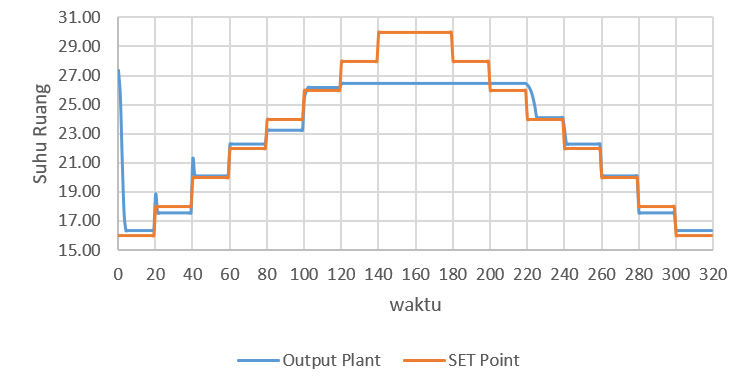
\includegraphics[width=0.75\textwidth]{figures/SimulinkTd}
	\caption{Grafik Hasil Simulasi Simulink untuk Suhu Ruang}
	\label{fig:5:SimulinkTd}
\end{figure}

\begin{figure}[!h]
	\centering
	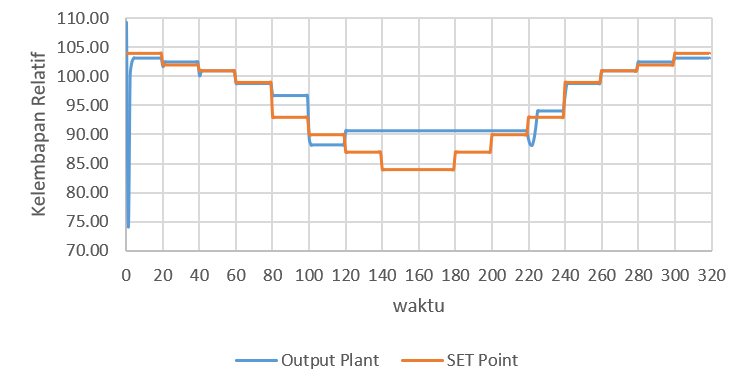
\includegraphics[width=0.75\textwidth]{figures/SimulinkRH}
	\caption{Grafik Hasil Simulasi Simulink untuk Kelembapan Relatif}
	\label{fig:5:SimulinkRH}
\end{figure}

\begin{figure}[!h]
	\centering
	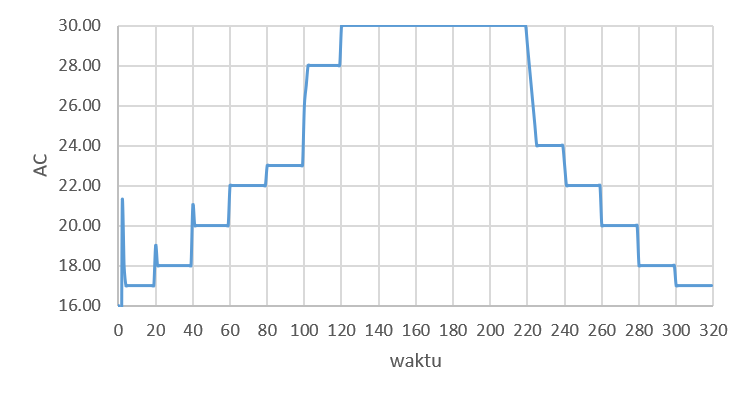
\includegraphics[width=0.75\textwidth]{figures/SimulinkAC}
	\caption{Grafik Variabel Manipulasi AC pada Simulasi Simulink}
	\label{fig:5:SimulinkAC}
\end{figure}

\begin{figure}[!h]
	\centering
	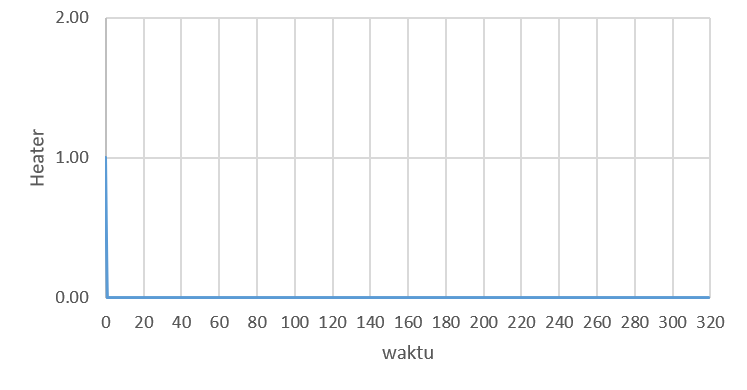
\includegraphics[width=0.75\textwidth]{figures/SimulinkHT}
	\caption{Grafik Variabel Manipulasi \textit{Heater} pada Simulasi Simulink}
	\label{fig:5:SimulinkHT}
\end{figure}
\vspace{1em}

Dengan meninjau nilai variabel manipulasi AC yang ditunjukkan pada Gambar \ref{fig:5:SimulinkAC}, dapat dilihat bahwa untuk mengendalikan suhu mencapai \textit{set point} 26$^\circ$C, perangkat AC perlu mengeluarkan sinyal sebesar 28$^\circ$C (waktu ke-100 hingga ke-120). Dengan demikian, ketika \textit{set point} bernilai 28$^\circ$C, perangkat AC hanya mampu mengeluarkan sinyal maksimum 30$^\circ$C (waktu ke-120 hingga ke-140).

Kurangnya kehandalan kinerja kontroler pada penelitian ini untuk mengendalikan suhu ruang di atas \textit{set point} 26$^\circ$C disebabkan oleh salah satu kelemahan model JST dalam pemodelan \textit{plant}. Secara fisis, proses pemanasan pada sistem bangunan (dalam hal ini \textit{climate chamber}) membutuhkan waktu yang cukup lama. Dengan demikian, proses pemanasan pada kenyataannya tetap bisa mencapai \textit{set point} suhu di atas 26$^\circ$C. Hanya saja proses tersebut membutuhkan waktu (\textit{settling time}) yang cukup lama. Akan tetapi, proses tersebut tidak dapat disimulasikan secara sempurna pada penelitian ini dikarenakan model JST \textit{plant} yang dibangun oleh Tri Hartanto\cite{skripsiTanto} hanya berupa model pasangan data dan bukan berupa model yang bergantung terhadap waktu. Sehingga, model JST \textit{plant} hanya dapat langsung mengeluarkan suatu nilai keluaran setiap menerima nilai masukan.

Ditinjau dari \textit{set point} 16$^\circ$C hingga 26$^\circ$C, didapatkan nilai \textit{steady-state error} untuk suhu ruang sebesar 0,15$^\circ$C pada proses pemanasan dan sebesar 0,2$^\circ$C pada proses pendinginan. Lalu, didapatkan pula nilai \textit{steady-state error} untuk kelembapan relatif sebesar 0,05\% pada proses pemanasan dan sebesar 0,02\% pada proses pendinginan. Sehingga rerata nilai \textit{steady-state error} sebesar 0,18$^\circ$C untuk suhu ruang dan sebesar 0,04\% untuk kelembapan relatif.